\documentclass[a4paper,12pt,oneside]{book}

\usepackage{graphicx} % to set the title_page image (university's logo)
\usepackage{url}
\usepackage{cite}     % bibliography

\usepackage{listings} % makes code look good
\usepackage{color}    % for syntax highlight

% this part defines how to do syntax highlight
\definecolor{dkgreen}{rgb}{0,0.6,0}
\definecolor{gray}{rgb}{0.5,0.5,0.5}
\definecolor{mauve}{rgb}{0.58,0,0.82}

\lstset{frame=tb,
  language=C++,
  aboveskip=0mm,
  belowskip=0mm,
  showstringspaces=false,
  columns=flexible,
  basicstyle={\small\ttfamily},
  numbers=none,
  numberstyle=\tiny\color{gray},
  keywordstyle=\color{blue},
  commentstyle=\color{dkgreen},
  stringstyle=\color{mauve},
  breaklines=true,
  breakatwhitespace=true
  tabsize=3
}
%end syntax highlight

%Automatically add contents
\newcommand\chap[1]{
  \chapter*{#1}
  \addcontentsline{toc}{chapter}{\protect\numberline{}#1}}


\title{Development of QR Codes based localization system}
\author{Giovanni De Francesco}

\begin{document}
  \begin{titlepage}
  \pagestyle{empty}

  \begin{center}
    {\bfseries\Large {\huge U}NIVERSITY OF {\huge T}RENTO}

    \vspace{0.2cm}

    {\large Department of Information Engineering and Computer Science}

    \vspace{0.5cm}

    \begin{center}
      
\includegraphics[width=0.3\textwidth]{img/logo_unitn.png}
    \end{center}

    \vspace{0.5cm}

    {\Large Degree course in Computer Science}

    \vspace{0.2cm}
    \line(1,0){338}
    \vspace{0.5cm}

    {\Large Final Thesis}

    \vspace{2.0cm}

    {\Large \bfseries {Development of localization system based on QR Codes recognition}}

    \vspace{0.3cm}
    

    \large
    \begin{center}
      \begin{tabular}{lcl}
        Supervisor: & \hspace{4cm} &  \hspace{1.5cm} Graduant: \\
        {\bfseries Prof. Luigi Palopoli} & \hspace{2cm} & {\bfseries Giovanni De Francesco } \\ \\
        Co-Supervisor: \\ {\bfseries Dott. Federico Moro}
      \end{tabular}
    \end{center}
    \vspace{2.0cm}

    {\large \bfseries Academic year 2013-2014}
    \vfill

  \end{center}

\end{titlepage}

  \thispagestyle{empty}
\begin{flushright}
\vspace*{3.0cm}
{\large \textit{A mio nonno Emilio e mia nonna Angela,}} \\ 
{\large \textit{gli angeli viventi che mi hanno accompagnato fin qui.}} \\ 
\end{flushright}

  \frontmatter
  	\tableofcontents
    \chapter{Abstract}

Indoor Localization Systems are currently being investigated by various companies and universities.
Uses of them are multiple and can lead to a market of 2.6 billion dollars \cite{market}.


  \mainmatter
    \chapter{An overview}

\vspace{0.5cm}
\section{The DALi project}

\vspace{1cm}
\begin{center}
      
\includegraphics[width=0.3\textwidth]{img/Dali-logo.png}
\end{center}
\vspace{1cm}

In modern times the world moves forward with incredible speed and creates new buildings aimed to engage people who use them, but often these environments are designed for adults with fully developed psychological and physical capabilities.
People who don't have the necessary requirements to navigate properly these new places begin to feel unsafe and perceive the world around even with hostility, which led to a confinement in buildings they know and trust.
This confinement, which became like a prison, reduces a variety of chances, such as: physical exercise, the gathering of fresh food and the making of social activities.
\newline
A specific subset of people who experience this kinds of problems every day are elders and, in order to provide help for this part of population, DALi is researching new technology which can effectively impact on their quality of living.
\newline
The major focus of the project at the moment of writing is a rollator which can help both the psychological sphere, by providing freedom of movement in newly discovered places to the user, and the physical one by actually aiding him during actual movements.

\newpage
\section{Role of the thesis inside DALi}
\vspace{0.5cm}
Designing and building a rollator brings many challenges in the robotic field, and even in the human computer interaction one, which are very interesting but, at the same time, they may reveal very difficult to develop. 
In fact, at the core of the rollator's functionalities there is a localization system which can track the user's movements in order to guide the person to his destination.
The precision requirement of the above mentioned unit, is an extremely delicate matter and needed further investigation in order to bring the best possibilities while limiting the error.
Therefore the work described on the next pages explores the possibility of building an environment where qr-codes provide information about the position and the trajectory to the rollator which can translate them in actual guidance for the user.






  

    \chapter{Problem description}

The main goals that must be achived by the new rollator is the navigation of the user inside an unfamiliar places without sacrificing the normal support and familiarity that a common rollator already gives.

\vspace{1cm}
\begin{center}
	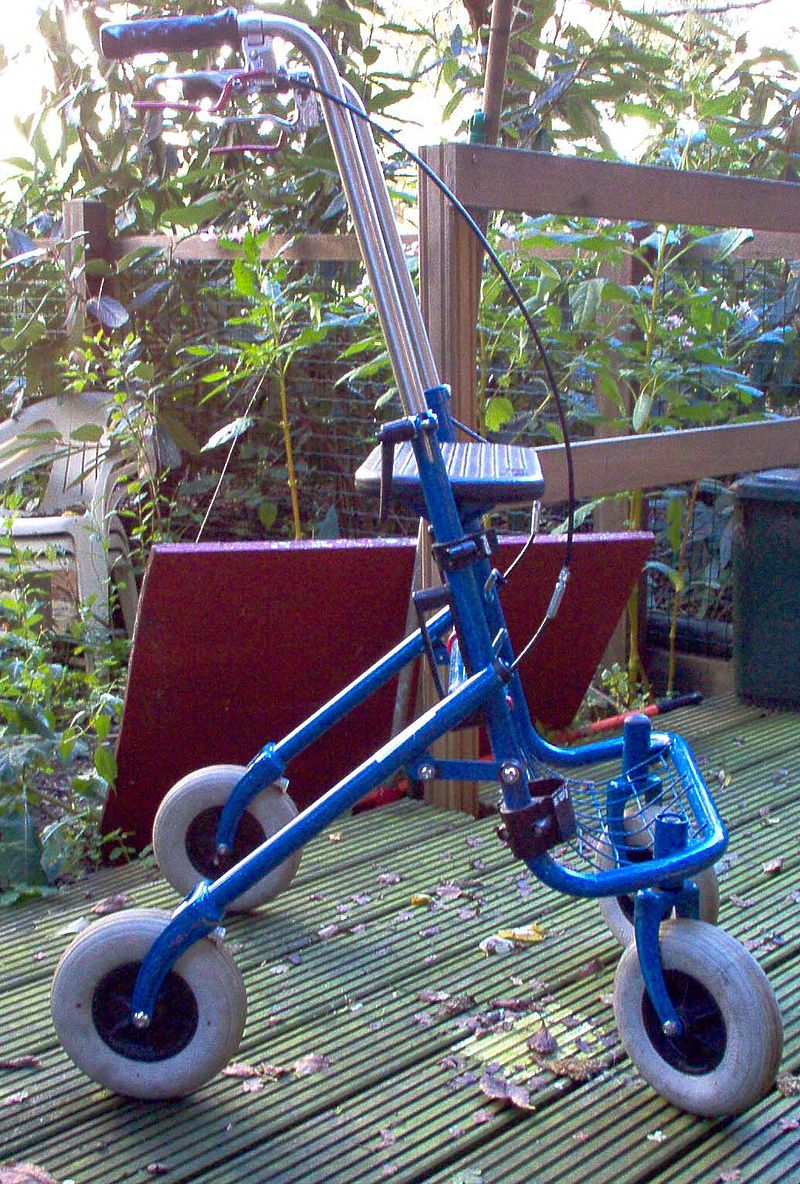
\includegraphics[width=0.3\textwidth]{img/rollator-old.jpg}    
\end{center}
\begin{center}
	The first rollator invented by Aina Wifalk \cite{imgrollator}  
\end{center}
\vspace{1cm} 










  

    \chapter{Tools}
\vspace{6cm}
Developing this kind of systems is extremely complex, as can be seen from the above analysis, but it would be a lot harder without algorithms and libraries made by other people.
In order to make our solution clearer and honor their work, in the following paragraphs I will briefly describe all the tools used by our project.
\newpage

\section{Language}
Every algorithm is implemented in C++ and all the used libraries bindings are also in that same language because performance is a must for these situations.   

\section{Developing environment}
A common laptop with the following specifications:
\begin{itemize}
  \item A 2,5 GHz Intel core i7 processor
  \item 8gb of RAM
  \item Integrated graphic card
\end{itemize}
and Slackware Linux -current as Operating System.


\section{The camera}
\begin{figure}[hbt]
    \vspace{1cm}
    \centering
    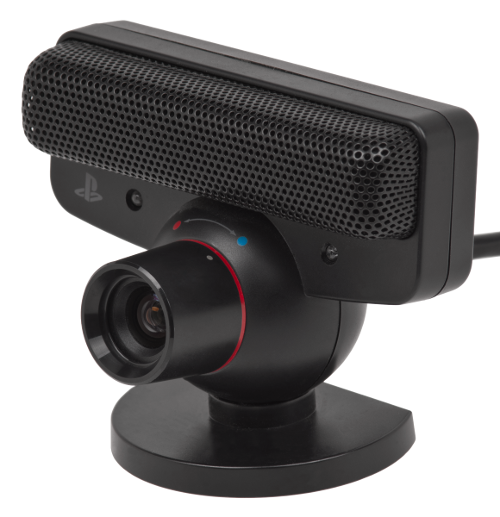
\includegraphics{img/pseye.png}
    \vspace{1cm}
\end{figure}

In order to stream videos or take pictures a Playstation 3 Eye has been used.
This camera can operate at 120Hz with a resolution of 320x240 pixels but we, instead, preferred to operate at 640x480 pixels with a frequency of 60Hz.
The device is automatically recognized and used without issues if the version of the Linux Kernel installed is later than the version 2.6.32 .
 

\section{Libraries}

\subsection{OpenCV}
This is the library which empower almost any device with a camera to process images and videos allowing manipulations with consolidated algorithms created by universities and companies in order to let the developer focus on their own solution of a problem.
In fact, OpenCV is the de facto standard for computer vision and it is wide-used in Sony Cameras for examples, but also on Android smartphones and iOS devices. 
\newline Used version: \textbf{2.4.9}

\subsection{ZBar}

The capability of decoding a QRCode is given by the ZBar library, which is open source and can decode also other kind of markers, for example: EAN-13/UPC-A, UPC-E, EAN-8 and Code 128.In addition, it is able to decode from a multitude of sources such as still images, raw intensity sensors and not only from video streams as the project shows. At the core of this possibility there is a streamlined implementation of the \textbf{ISO/IEC 18004:2000} encoding/decoding RFC in C which is perfect for embedded purposes.
\newline Used version: \textbf{0.10}.

\subsection{Eigen}
This library provide abstractions and utilities for linear algebra such as numerical solvers but also matrices and related algorithms which are the very one used by our project.
The whole code is free-software because it is licensed with MPLv2 and it is based on C++ templating system, in this way the developer can use only the needed header file which allows reasonable compilation time and flexibility.\cite{eigeninfo}
\newline Used version: \textbf{3.2.1}.

\section{Other algorithms}

\subsection{Rectification}
The image rectification process removes the perspectiveand corrects distorsion inside an image.
This method creates a new flat image as shown in the figures below:




 

    % \chapter{The algorithm}

I produced a class which abstracts a QRCode and defines various methods to access the desired properties. This class was declared in a .h file and implemented in .cpp file as the standards wants, in addition, the structure of this code is designed with developers in mind.In fact after the constructor call, no other parameters are needed to make the class work and, after a QRCode object is instantiated, the user can directly call all \textbf{get\textunderscore{}\emph{propertyname}()} methods and use their results for its own purposes. However, this design, connected with the fact that the rectification algorithm requires many parameters, produced a pretty long constructor signature which is not very beautiful to see and use. However, even if the code has to run on embedded devices, the rest of the code tries to stay as elegant as possible because someone else could feel the need to understand and modify it.
In addition the codebase concerning the algorithm implementation is very small and it counts about 360 lines of code. Although, all the testing and benchmarking software required more than one thousand additional lines of code.

\section{ZBar's recognition improvement} 
No software is perfect and considering that ZBar is just at 0.10 version at the moment indicates how far from perfection is. Furthermore, for our purposes, its capability to recognize QRCode was just sufficient and needed some tuning in order to be used.To achieve this result, a great number of experiments was required and more than 400 pictures of QRCodes with different light conditions and angles has been taken. Moreover, this lead to the development of a process consisting in seven incremental steps which makes use of different elaborations on the picture before sending it to the ZBar's API.
\newpage
In particular, these are all different tryings that the method \textbf{searchQRCode()} does:

\begin{enumerate}
	\item The basic greyscale picture taken by the camera.
	\item An image rotated by 180 degrees
	\item A only black and white image (called also: filter).
	\item A rectified image
	\item A rectified and filtered image
	\item A rectified and rotated image
	\item A rectified, filtered and rotated image.
\end{enumerate}

In our experiments on the last set of 220 images, ZBar alone was able to detect 142 QRCodes whilst the process lead to the recognition of 169. Moreover, the second passage helped in 8 cases, the third package in 11, the forth in 4 cases and the last passage on the other 4. In fact, we noticed that ZBar have some problem to recognize QRCodes inclined with an angle from 180 to 360 degrees.
As can be seen, there are two problems in the process: steps five and six weren't useful and still 51 QRCodes couldn't be found. However, the first problem is there for the reason that those steps are sub-cases of the seventh try, and we suppose that under certain circumstances they could be helpful, instead, the reason behind the second problem was found by checking each image which showed it. Furthermore, the problem was that those markers were too far from the camera even if the photo could contain them.

\section{Reduce trajectory approximation}
The rollator 


    % \chapter{Accuracy tests and results}

Every test has been conducted with a camera positioned at 75 centimeters from the ground, with an inclination of 24.6 degrees. Furthermore, the webcam's field of view is approximatively 90 centimeters wide and almost 40 centimeters tall. QRCodes are placed on a 3x3 grid, in addition, their id is assigned from left to right and from the bottom to the top, as shown in figure \ref{field}.

\begin{figure}[hbt]
    \centering
    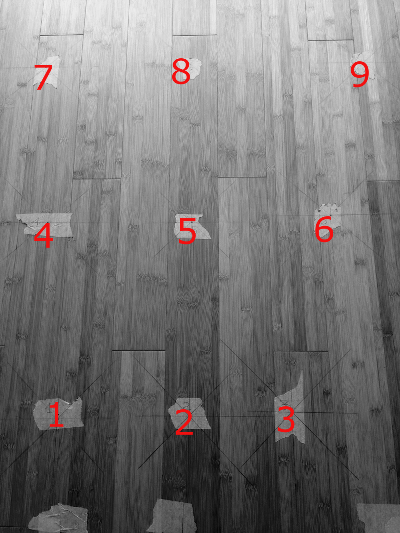
\includegraphics[scale=0.5]{img/field.png}
    \caption{QRCode's grid system. \label{field}}
\end{figure}

Moreover, in order to increase the number of tests using the same resources, three pictures for each angle was taken in every location. The orientations taken into account range from 0 to 360 degrees with an increment of 45 degrees in each step. Therefore, these tests was made on a basis of 216 pictures.
\newline
The positions of every marker was measured and they were hard-coded into the program in order to run the proposed software. As can be seen, Table \ref{qrpos} contains coordinates x and y in centimeters for every QRCode's id.

\begin{center}
	\label{qrpos}
  \begin{tabular}{ | l | l | l |}
    \hline
    id & pos\textunderscore x & pos\textunderscore y \\ \hline
    1 & 18.5 & 22 \\ \hline
    2 & 19 & 0 \\ \hline
    3 & 20 & -18 \\ \hline
    4 & 54 & 28 \\ \hline
    5 & 54 & 0 \\ \hline
    6 & 54 & -28 \\ \hline
    7 & 91 & 31 \\ \hline
    8 & 91 & 0 \\ \hline
    9 & 91 & -37 \\ \hline
  \end{tabular}
\end{center}
    % \input{chapter_6}
    % \chapter{Conclusions}

This thesis describes a method to estimate the position of a QRcode inside a configured environment.
The dissertation stated the need of this particular application at the beginning and continued with an analysis of the tools used. Afterwards, the thesis explained the solving algorithm leading to the demonstration of its capability with tests. Therefore, these results look promising and can be used as a base to build an indoor step-by-step navigator. In particular, this was done with the goal to free elders of their frighten of new and crowded place as stated by the DALi project. Furthermore, this system is actually being used on a testing rollator, in order to discover its ability to let a user explore an unfamiliar environment. All the code is public on my GitHub's \footnote{ \url{http://github.com/jibbo/qrlocalization-thesis} } account and it is released under the license Creative Commons CC BY-NC 4.0 \footnote{\url{http://creativecommons.org/licenses/by-nc/4.0/}} and any form of redistribution is welcomed as far as DALi is mentioned and credited.\newline
Future work might include:
\begin{itemize}
	\item Find and solve the problem with ZBar recognition which appears when a QRCode has certain orientations. This would improve the whole system capabilities.
	\item Improvements on the rectification algorithm are needed in order to remove duplicate code.
	\item Make experiments with QRCodes printed with \textbf{invisible ink} and an infrared camera, in order to free the system by light problems and paper's decay giving by usage. 
\end{itemize}       
  \chapter*{Acknowledgements}
\thispagestyle{empty}

I would like to thank my supervisors Luigi Palopoli and Federico moro who helped me every time I had fallen during the writing of the algorithm.
\\
Many thanks to David Macii whose support and guidance was very helpful.
\\ \\
My gratitude goes also to my girlfriend Giulia, my family and my roommate Federico who all were there for me in dark moments.
\\ \\
In addition, I am pleased to acknowledge all the friends who stayed at my side in these three years:
Giulio Fornasaro, Luca Zamboni and Roberto Zen but also Andrea Cristiano, Andrea Panizza and Lorenzo Lotto with all the other course mates, because, without them, this time would have been more boring.


  \bibliographystyle{unsrt}
  \bibliography{bibliography}
\end{document}
